\section{Advanced Particle Filters}\label{sec:particle_filtering}

\subsection{Particle Filter}

The SIR resamples at every time step, which eliminates weight degeneracy but introduces unnecessary computational cost when weights are already well-distributed. The generic particle filter (PF), presented in \Cref{alg:PF}, improves upon the SIR by resampling only when a certain criterion is met. The most common criterion is based on the effective sample size:
\begin{equation}
	N_{eff}\triangleq\frac{N}{1+\mathbb{V}_q\left[\dfrac{p\left(\mathbf{x}_{0:k}^{(i)}|\mathbf{z}_{1:k}\right)}{q\left(\mathbf{x}_{0:k}^{(i)}|\mathbf{z}_{1:k}\right)}\right]}
\end{equation}

When all the weights are equally distributed, the variance is zero, and thus $N_{eff}=N$. Conversely, $N_{eff}\to1$ in the fully degenerate case. While this quantity is not directly computable, it can be estimated by:
\begin{equation}
	\hat{N}_{eff}\triangleq\frac{1}{\displaystyle\sum_{i=1}^N\left(w_k^{(i)}\right)^2}\leq N
\end{equation}

Thanks to this metric, the PF only performs the resampling step when:
\begin{equation}
	\hat{N}_{eff}<N_{th}
\end{equation}
where $N_{th}$ is a predetermined threshold value, typically chosen proportional to $N$.

\begin{algorithm}[ht]
	\begin{algorithmic}
	\State{$\forall i\in[\![1,N]\!],\:x_k^{(i)}\sim q\left(\cdot|x_{k-1}^{(i)},z_k\right)$}\Comment{Particle propagation}
	\State{$\forall i\in[\![1,N]\!],\:\tilde{w}_k^{(i)}=w_{k-1}^{(i)}\:\dfrac{\tilde{p}\left(z_k|x_k^{(i)}\right)\:\tilde{p}\left(x_k^{(i)}|x_{k-1}^{(i)}\right)}{\tilde{q}\left(x_k^{(i)}|\mathbf{x}_{0:k-1}^{(i)},\mathbf{z}_{1:k}\right)}$}\Comment{Weight update}
	\State{$\displaystyle\forall i\in[\![1,N]\!],\:w_k^{(i)}=\left.\tilde{w}_k^{(i)}\middle/\sum_{j=1}^N\tilde{w}_k^{(j)}\right.$}\Comment{Normalisation}
	\State{$\displaystyle\hat{N}_{eff}=\left.1\middle/\sum_{i=1}^N\left(w_k^{(i)}\right)^2\right.$}\Comment{Resampling criterion}
	\If{$\hat{N}_{eff}<N_{th}$}
	\State{$\left\{x_k^{(j)},w_k^{(j)},-\right\}_{j=1}^N\gets\textup{Resampling}\left(\left\{x_k^{(i)},w_k^{(i)}\right\}_{i=1}^N\right)$}\Comment{Resampling}
	\EndIf
	\State{$\displaystyle\hat{x}_k=\sum_{j=1}^Nw_k^{(j)}\varphi\left(x_k^{(j)}\right)$}\Comment{State estimation}
	\State{$\displaystyle P_k=\sum_{j=1}^Nw_k^{(j)}\left(\varphi\left(x_k^{(j)}\right)-\hat{x}_k\right)\left(\varphi\left(x_k^{(j)}\right)-\hat{x}_k\right)^\top$}\Comment{State covariance}
	\end{algorithmic}\caption{Particle Filter}\label{alg:PF}
\end{algorithm}

Though resampling resolves weight degeneracy, it introduces a new issue, called particle impoverishment. Indeed, after resampling, particles with high weights are replicated multiple times, while those with low weight are discarded. As a result, multiple particles collapse to a single point in the state-space. This loss of particle diversity is particularly severe in low evolution noise or high-dimensional settings, as little diversity is re-introduced at the propagation step. This phenomenon is illustrated by \Cref{fig:impoverishment}.

\begin{figure}[ht]
	\centering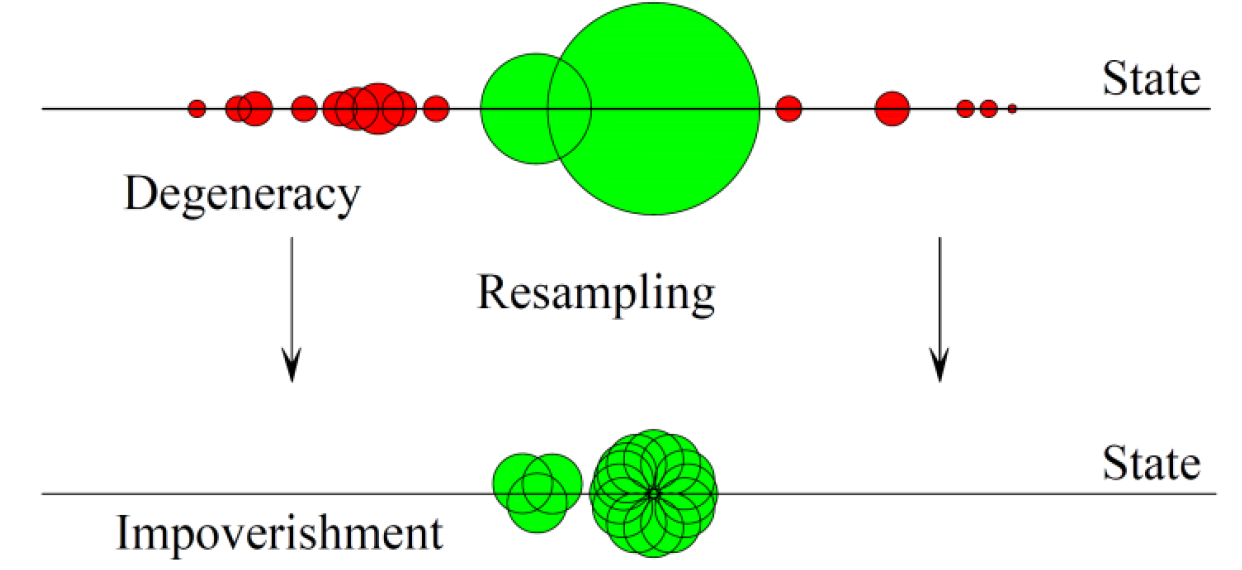
\includegraphics[width=0.6\textwidth]{figures/particle_impoverishment.png}
	\caption{The resampling step is triggered when a small subset of particles hold most of the total mass. After resampling, most of the negligible particles are discarded, while the heavier particles are duplicated into many new ones. By eliminating lighter particles, the effective support of the empirical approximation shrinks, reducing the ability of the PF to represent diffuse or multimodal regions of the PDF, and ultimately degrading long-term exploration of the state space.}\label{fig:impoverishment}
\end{figure}

\subsection{Regularised Particle Filter}

The regularised particle filter (RPF) addresses particle impoverishment by replacing the discrete empirical measure $S^N$ of \Cref{th:empirical_measure} with a continuous kernel mixture after resampling. The idea behind this is to use kernel density estimation to expand the support of the approximated density and restore particle diversity, as shown in \Cref{fig:regularisation}. This is formally introduced by \Cref{th:regularisation_kernel,th:KDE}.

\begin{figure}[ht]
	\centering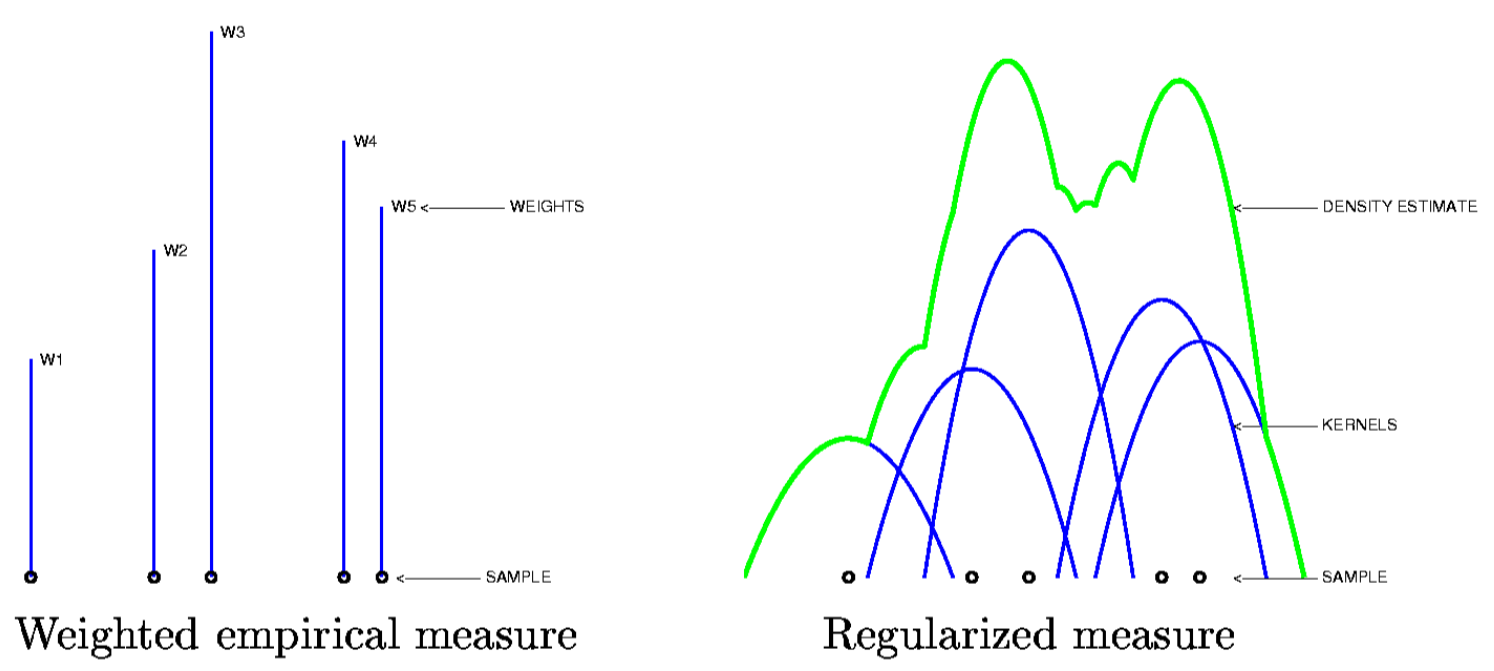
\includegraphics[width=0.8\textwidth]{figures/regularisation.png}
	\caption{Instead of approximating the PDF by a mixture of Dirac distributions $\displaystyle p(x_k|\mathbf{z}_{1:k})\:dx\approx\sum_{i=1}^Nw_k^{(i)}\:\delta\left(x_k-X_k^{(i)}\right)$, the RPF approximates it by a mixture of smooth kernels $\displaystyle p(x_k|\mathbf{z}_{1:k})\approx\sum_{i=1}^Nw_k^{(i)}\:\mathcal{K}_h\left(x_k-X_k^{(i)}\right)$. New particles are drawn from this continuous approximation rather than from the discrete set, which restores diversity.}\label{fig:regularisation}
\end{figure}

\begin{definition}[Regularisation kernels]\label{th:regularisation_kernel}
	Let $K:\mathbb{R}^{d_x}\to\mathbb{R}$. $K$ is a regularisation kernel if:
	\begin{equation}
		\left\{\begin{array}{ll}
		\forall x\in\mathbb{R}^{d_x},\:K(x)\geq0&\text{positive}\\
		\forall x\in\mathbb{R}^{d_x},\:K(-x)=K(x)&\text{symmetric}\\
		\displaystyle\int{K(x)\:dx}=1&\text{normalised}\\
		\displaystyle\int{\|x\|^2K(x)\:dx}<\infty&\text{of finite variance}
		\end{array}\right.
	\end{equation}

	Furthermore, for $K$ a regularisation kernel and $h>0$, we define the rescaled kernel $K_h$ of bandwidth $h$ as:
	\begin{equation}
		K_h:\left\{\begin{aligned}
		\mathbb{R}^{d_x}&\to\mathbb{R}^{d_x}\\
		x&\mapsto\frac{1}{h^{d_x}}K\left(\frac{x}{h}\right)
		\end{aligned}\right.
	\end{equation}
\end{definition}

\begin{definition}[Regularised estimator]\label{th:KDE}
	Let $*$ denote the convolution operator. The regularised measure $S_{K_h}^N$ of some empirical measure $S^N$ is:
	\begin{equation}
		S_{K_h}^N(\mu)\triangleq K_h*S^N(\mu)
	\end{equation}

	In particular, the regularised self-normalised estimator verifies:
	\begin{equation}
		\tilde{S}_{K_h}^N(\mu,\nu)=\sum_{i=1}^Nw^{(i)}\:\left(K_h*\delta_{X^{(i)}}\right)
	\end{equation}
	and the corresponding estimator is:
	\begin{equation}
		\left\langle\tilde{S}_{K_h}^N(\mu,\nu),\varphi\right\rangle=\sum_{i=1}^Nw^{(i)}\:\left(K_h*\varphi\right)\left(X^{(i)}\right)
	\end{equation}
	by symmetry of $K$.
\end{definition}

The choice of bandwidth $h$ is critical to the performance of the RPF. If $h$ is too small, $K_h$ concentrates around the Dirac measure, and the regularisation has no practical effect on particle diversity. Conversely, the kernel density estimate over-smooths the posterior when $h$ is too large, artificially spreading particles across regions of low probability, and degrading filter accuracy. In this section, we present two classical choices for $K_h$:
\begin{itemize}
	\item\textbf{Epanechnikov kernel.} When the prior $p$ is Gaussian, and the covariance matrix is equal to the identity, this kernel is optimal in the mean integrated squared error (MISE). It is defined by:
	\begin{equation}
		\left\{\begin{aligned}
		K_{Epa}&:x\mapsto\frac{d_x+2}{2c_{d_x}}\left(1-\|x\|^2\right)\mathbbm{1}_{\|x\|\leq1}(x)\\
		h_{Epa}&=\left(\frac{8(d_x+4)\left(2\sqrt{\pi}\right)^{d_x}}{c_{d_x}}\right)^{\frac{1}{d_x+4}}N^{-\frac{1}{d_x+4}}
		\end{aligned}\right.
	\end{equation}
	where:
	\begin{equation}
		c_{d_x}=\frac{\pi^{d_x/2}}{\Gamma(d_x/2+1)}
	\end{equation}
	is the volume of the $\mathbb{R}^{d_x}$ unit sphere, and $\Gamma$ is the Gamma function.
	\item\textbf{Gaussian kernel.} While suboptimal with respect to the Epanechnikov kernel, it is simpler to compute. Its expression is given by:
	\begin{equation}
		\left\{\begin{aligned}
		K_{Gauss}&:x\mapsto(2\pi)^{-d_x/2}\text{exp}\left(-\frac{\|x\|^2}{2}\right)\\
		h_{Gauss}&=\left(\frac{4}{d_x+2}\right)^{\frac{1}{d_x+4}}N^{-\frac{1}{d_x+4}}
		\end{aligned}\right.
	\end{equation}
\end{itemize}

It must be noted that the assumptions for the Epanechnikov, and consequently the Gaussian, regularisation are not usually met in practice. Indeed, the estimated covariance matrix $P_k$ is not always equal to $I$. To solve this issue, a whitening step is performed before the regularisation, during which every particle is replaced by $A_k^{-1}\:x_k^{(i)}$, where $A_k$ is the square root of $P_k$ with respect to the Cholesky factorisation:
\begin{equation}
	A_kA_k^\top=P_k
\end{equation}

This ensures that the covariance matrix of the new particle set is the identity. While seemingly computationally heavy, this reduces to using the following regularisation kernel on the standard particle set:
\begin{equation}
	\tilde{K}_h:x\mapsto\frac{\text{det}(A_k)^{-1}}{h^{d_x}}K\left(\frac{1}{h}A_k^{-1}x\right)
\end{equation}
Moreover, the bandwidth $h$ is multiplied by a modulation factor $\alpha_{reg}\in[0,1]$ to avoid over-smoothing in cases where the PDF is multimodal. The pseudo-code for the RPF is given by \Cref{alg:RPF}.

\begin{algorithm}[ht]
	\begin{algorithmic}
	\State{$\forall i\in[\![1,N]\!],\:x_k^{(i)}\sim q\left(\cdot|x_{k-1}^{(i)},z_k\right)$}\Comment{Particle propagation}
	\State{$\forall i\in[\![1,N]\!],\:\tilde{w}_k^{(i)}=w_{k-1}^{(i)}\:\dfrac{\tilde{p}\left(z_k|x_k^{(i)}\right)\:\tilde{p}\left(x_k^{(i)}|x_{k-1}^{(i)}\right)}{\tilde{q}\left(x_k^{(i)}|\mathbf{x}_{0:k-1}^{(i)},\mathbf{z}_{1:k}\right)}$}\Comment{Weight update}
	\State{$\displaystyle\forall i\in[\![1,N]\!],\:w_k^{(i)}=\left.\tilde{w}_k^{(i)}\middle/\sum_{j=1}^N\tilde{w}_k^{(j)}\right.$}\Comment{Normalisation}
	\State{$\displaystyle\hat{N}_{eff}=\left.1\middle/\sum_{i=1}^N\left(w_k^{(i)}\right)^2\right.$}\Comment{Resampling criterion}
	\If{$\hat{N}_{eff}<N_{th}$}
	\State{$\displaystyle\hat{x}_k=\sum_{i=1}^Nw_k^{(i)}\varphi\left(x_k^{(i)}\right)$}\Comment{Whitening}
	\State{$\displaystyle P_k=\sum_{i=1}^Nw_k^{(i)}\left(\varphi\left(x_k^{(i)}\right)-\hat{x}_k\right)\left(\varphi\left(x_k^{(i)}\right)-\hat{x}_k\right)^\top$}
	\State{$A_k\text{ s.t. }A_kA_k^\top=P_k$}
	\State{$\left\{x_k^{(j)},w_k^{(j)},-\right\}_{j=1}^N\gets\textup{Resampling}\left(\left\{x_k^{(i)},w_k^{(i)}\right\}_{i=1}^N\right)$}\Comment{Resampling}
	\State{$\forall j\in[\![1,N]\!],\:\varepsilon^{(j)}\sim K$}\Comment{Regularisation}
	\State{$\forall j\in[\![1,N]\!],\:x_k^{(j)}\gets x_k^{(j)}+\alpha_{reg}hA_k\:\varepsilon^{(j)}$}
	\EndIf
	\State{$\displaystyle\hat{x}_k\gets\sum_{j=1}^Nw_k^{(j)}\varphi\left(x_k^{(j)}\right)$}\Comment{State estimation}
	\State{$\displaystyle P_k\gets\sum_{j=1}^Nw_k^{(j)}\left(\varphi\left(x_k^{(j)}\right)-\hat{x}_k\right)\left(\varphi\left(x_k^{(j)}\right)-\hat{x}_k\right)^\top$}\Comment{State covariance}
	\end{algorithmic}\caption{Regularised Particle Filter}\label{alg:RPF}
\end{algorithm}

\subsection{Auxiliary Particle Filter}

The auxiliary particle filter (APF) addresses the degeneracy problem at its root by exploiting a different weakness of the SIR. Since particles are propagated before the new observation $z_k$ is taken into account, particles that will ultimately receive low likelihood waste computational effort. The APF thus introduces a look-ahead step by using a prediction of their future likelihood to resample promising parent particles before propagation.

Formally, the APF targets the joint distribution $p(x_k,i|\mathbf{z}_{1:k})$, where $i\in[\![1,N]\!]$ indexes the parent particle at time $k-1$. Using Bayes' theorem and the law of total probability gives:
\begin{equation}
	p(x_k,i|\mathbf{z}_{1:k})\propto p(z_k|x_k,i,\mathbf{z}_{1:k-1})\:p(x_k|i,\mathbf{z}_{1:k-1})\:p(i|\mathbf{z}_{1:k-1})\label{eq:joint_distribution_APF}
\end{equation}

Each term of this decomposition can be simplified as follows:
\begin{itemize}
	\item\Cref{th:observation_independence} states that the current observation depends only on the current state:
	\begin{equation}
		p(z_k|x_k,i,\mathbf{z}_{1:k-1})=p(z_k|x_k)
	\end{equation}
	\item Since the parent index uniquely determines the ancestor trajectory, conditioning on $i$ is equivalent to conditioning on $x_{0:k-1}^{(i)}$. Moreover, \Cref{th:Markov} establishes that $(x_k)_{k\geq0}$ is a Markov chain, and thus:
	\begin{equation}
		p(x_k|i,\mathbf{z}_{1:k-1})=p\left(x_k|\mathbf{x}_{0:k-1}^{(i)},\mathbf{z}_{1:k-1}\right)=p\left(x_k|x_{k-1}^{(i)}\right)
	\end{equation}
	\item Finally, assuming that the particle approximation is exact gives:
	\begin{equation}
		p(i|\mathbf{z}_{1:k-1})\propto w_{k-1}^{(i)}
	\end{equation}
\end{itemize}

Combining these equations reduces \eqref{eq:joint_distribution_APF} to:
\begin{equation}
	p(x_k,i|\mathbf{z}_{1:k})\propto p\left(z_k|x_k\right)\:p\left(x_k|x_{k-1}^{(i)}\right)\:w_{k-1}^{(i)}
\end{equation}

However, $p(z_k|x_k)$ cannot be evaluated before $x_k$ is drawn. It is thus approximated by $p\left(z_k|\mu_k^{(i)}\right)$, where:
\begin{equation}
	\mu_k^{(i)}\sim p\left(\cdot|x_{k-1}^{(i)}\right)
\end{equation}
is an auxiliary particle drawn from the transition density, and used to assess the consistency of the future particle $x_k^{(i)}$ with the new observation $z_k$. Therefore, the importance density is:
\begin{equation}
	q(x_k,i|\mathbf{z}_{1:k})\propto p\left(z_k|\mu_k^{(i)}\right)\:p\left(x_k|x_{k-1}^{(i)}\right)\:w_{k-1}^{(i)}
\end{equation}

Since they are drawn from the prior distribution, \eqref{eq:weight_update_prior} ensures that the auxiliary weights $\lambda_k^{(i)}$ follow:
\begin{equation}
	\lambda_k^{(i)}\propto w_{k-1}^{(i)}\:\tilde{p}\left(z_k|\mu_k^{(i)}\right)
\end{equation}

In the hope that the evolution noise is sufficiently weak for the auxiliary particles to correctly represent the future particle set, the parent indices $\left\{i^{(j)}\right\}_{j=1}^N$ are resampled according to the auxiliary weights.

The new particle set is then propagated through a standard SIS algorithm using the transition density:
\begin{equation}
	x_k^{(j)}\sim p\left(\cdot|x_{k-1}^{\left(i^{(j)}\right)}\right)
\end{equation}
with their weights updating as:
\begin{equation}
	\begin{aligned}
	w_k^{(j)}&\propto\frac{\tilde{p}\left(x_k,i^{(j)}|\mathbf{z}_{1:k}\right)}{\tilde{q}\left(x_k,i^{(j)}|\mathbf{z}_{1:k}\right)}\\
	&\propto\frac{\tilde{p}\left(z_k|x_k^{(j)}\right)\:\tilde{p}\left(x_k^{(j)}|x_{k-1}^{\left(i^{(j)}\right)}\right)\:w_{k-1}^{\left(i^{(j)}\right)}}{\tilde{p}\left(z_k|\mu_k^{\left(i^{(j)}\right)}\right)\:\tilde{p}\left(x_k^{(j)}|x_{k-1}^{\left(i^{(j)}\right)}\right)\:w_{k-1}^{\left(i^{(j)}\right)}}\\
	&\propto\frac{\tilde{p}\left(z_k|x_k^{(j)}\right)}{\tilde{p}\left(z_k|\mu_k^{\left(i^{(j)}\right)}\right)}
	\end{aligned}
\end{equation}

The full APF algorithm is given in \cref{alg:APF}.

\begin{algorithm}[ht]
	\begin{algorithmic}
	\State{$\forall i\in[\![1,N]\!],\:\mu_k^{(i)}\sim p\left(\cdot|x_{k-1}^{(i)}\right)$}\Comment{Auxiliary propagation}
	\State{$\forall i\in[\![1,N]\!],\:\tilde{\lambda}_k^{(i)}\propto w_{k-1}^{(i)}\:\tilde{p}\left(z_k|\mu_k^{(i)}\right)$}\Comment{Auxiliary update}
	\State{$\displaystyle\forall i\in[\![1,N]\!],\:\lambda_k^{(i)}=\left.\tilde{\lambda}_k^{(i)}\middle/\sum_{j=1}^N\tilde{\lambda}_k^{(j)}\right.$}\Comment{Normalisation}
	\State{$\left\{-,-,i^{(j)}\right\}_{j=1}^N=\textup{Resampling}\left(\left\{\mu_k^{(i)},\lambda_k^{(i)}\right\}_{i=1}^N\right)$}\Comment{Resampling}
	\State{$\forall j\in[\![1,N]\!],\:x_k^{(j)}\sim p\left(\cdot|x_{k-1}^{\left(i^{(j)}\right)}\right)$}\Comment{Particle propagation}
	\State{$\forall j\in[\![1,N]\!],\:\tilde{w}_k^{(j)}\propto\dfrac{\tilde{p}\left(z_k|x_k^{(j)}\right)}{\tilde{p}\left(z_k|\mu_k^{\left(i^{(j)}\right)}\right)}$}\Comment{Weight update}
	\State{$\displaystyle\forall j\in[\![1,N]\!],\:w_k^{(j)}=\left.\tilde{w}_k^{(j)}\middle/\sum_{i=1}^N\tilde{w}_k^{(i)}\right.$}\Comment{Normalisation}
	\State{$\displaystyle\hat{x}_k=\sum_{j=1}^Nw_k^{(j)}\varphi\left(x_k^{(j)}\right)$}\Comment{State estimation}
	\State{$\displaystyle P_k=\sum_{j=1}^Nw_k^{(j)}\left(\varphi\left(x_k^{(j)}\right)-\hat{x}_k\right)\left(\varphi\left(x_k^{(j)}\right)-\hat{x}_k\right)^\top$}\Comment{State covariance}
	\end{algorithmic}\caption{Auxiliary Particle Filter}\label{alg:APF}
\end{algorithm}

\begin{remark}[Comparison between the RPF and the APF]
	Both the RPF and the APF aim to alleviate the degeneracy and impoverishment problems of the standard PF. However, they do so differently. The RPF uses kernel density estimation to reintroduce diversity to the resampling step. Conversely, the APF avoids wasting particles by pre-selecting promising parents before propagation, and functions best when the evolution noise is small. This difference provides an empirical criterion for choosing between the two filters: the RPF is preferable in high evolution noise regimes, while the APF is better suited to nearly deterministic dynamics.
\end{remark}

\subsection{Rao-Blackwellised Particle Filter}

The Rao-Blackwellised particle filter (RBPF), also known as the marginalised particle filter, reduces the dimension of the
state-space explored by the particle filter by exploiting a partial linear-Gaussian structure in the state-space model. Suppose that the state can be decomposed as:
\begin{equation}
	x_k=\left[x_k^n,x_k^l\right]
\end{equation}
such that the dynamics of $x_k^l$ are linear and Gaussian conditionally on $x_k^n$. The navigation system \eqref{eq:navigation_problem} can be rewritten as:
\begin{equation}
	(S):\left\{\begin{aligned}
	x_k^n&=F_k^n\left(x_{k-1}^n\right)\:x_{k-1}^l+f_k^n\left(x_{k-1}^n\right)+w_k^n\\
	x_k^l&=F_k^l\left(x_{k-1}^n\right)\:x_{k-1}^l+f_k^l\left(x_{k-1}^n\right)+w_k^l\\
	z_k&=H_k\left(x_k^n\right)\:x_k^l+h_k\left(x_k^n\right)+n_k
	\end{aligned}\right.\label{eq:RBPF_model}
\end{equation}
with:
\begin{equation}
	w_k=\begin{bmatrix}w_k^n\\w_k^l\end{bmatrix}
	\sim\mathcal{N}\left(0,\begin{bmatrix}
	Q_k^n&Q_k^{nl}\\(Q_k^{nl})^\top&Q_k^l
	\end{bmatrix}\right),\quad n_k\sim\mathcal{N}(0,R_k)
\end{equation}
$x_0^n$ of known distribution, and $x_0^l$ Gaussian.

The idea behind the RBPF is to factorise the PDF as:
\begin{equation}
	p\left(x_k^l,x_k^n|\mathbf{z}_{1:k}\right)=p\left(x_k^l|x_k^n,\mathbf{z}_{1:k}\right)\:p\left(x_k^n|\mathbf{z}_{1:k}\right)
\end{equation}
where $p(x_k^n|\mathbf{z}_{1:k})$ is estimated via particle filtering techniques, and $p(x_k^l|x_k^n,\mathbf{z}_{1:k})$ is analytically solved by a Kalman filter.

When $Q_k^{nl}\neq 0$, the noises $w_k^l$ and $w_k^n$ are correlated, and the Kalman filter cannot be applied directly. To decouple them, we define the decorrelated noise:
\begin{equation}
	\overline{w}_k^l\triangleq w_k^l-Q_k^{nl}\:(Q_k^n)^{-1}\:w_k^n
\end{equation}
whose expectation is $0$, and its covariance is:
\begin{equation}
	\begin{aligned}
	\overline{Q}_k^l&\triangleq\mathbb{E}\left[\overline{w}_k^l\:{\overline{w}_k^l}^\top\right]\\
	&=\mathbb{E}\left[(w_k^l-Q_k^{nl}\:(Q_k^n)^{-1}\:w_k^n)\:(w_k^l-Q_k^{nl}\:(Q_k^n)^{-1}\:w_k^n)^\top\right]\\
	&=\mathbb{E}\left[w_k^l\:(w_k^l)^\top\right]-\mathbb{E}\left[w_k^l\:(Q_k^{nl}\:(Q_k^n)^{-1}\:w_k^n)^\top\right]-\\
	&\qquad\mathbb{E}\left[(Q_k^{nl}\:(Q_k^n)^{-1}\:w_k^n)\:(w_k^l)^\top\right]+\mathbb{E}\left[(Q_k^{nl}\:(Q_k^n)^{-1}\:w_k^n)\:(Q_k^{nl}\:(Q_k^n)^{-1}\:w_k^n)^\top\right]\\
	&=\mathbb{E}\left[w_k^l\:(w_k^l)^\top\right]-\mathbb{E}\left[w_k^l\:(w_k^n)^\top\right](Q_k^n)^{-\top}\:(Q_k^{nl})^\top-\\
	&\qquad Q_k^{nl}\:(Q_k^n)^{-1}\:\mathbb{E}\left[w_k^n\:(w_k^l)^\top\right]+Q_k^{nl}\:(Q_k^n)^{-1}\:\mathbb{E}\left[w_k^n\:(w_k^n)^\top\right]\:(Q_k^n)^{-\top}\:(Q_k^{nl})^\top\\
	&=Q_k^l-Q_k^{nl}\:(Q_k^n)^{-\top}\:(Q_k^{nl})^\top-Q_k^{nl}\:(Q_k^n)^{-1}\:(Q_k^{nl})^\top+Q_k^{nl}\:(Q_k^n)^{-1}\:Q_k^n\:(Q_k^n)^{-\top}\:(Q_k^{nl})^\top\\
	&=Q_k^l-Q_k^{nl}\:(Q_k^n)^{-1}\:Q_k^{nl}-Q_k^{nl}\:(Q_k^n)^{-1}\:Q_k^{nl}+Q_k^{nl}\:(Q_k^n)^{-1}\:Q_k^{nl}\\
	&=Q_k^l-Q_k^{nl}\:(Q_k^n)^{-1}\:Q_k^{nl}
	\end{aligned}
\end{equation}

Computing:
\begin{equation}
	\begin{aligned}
	\mathbb{E}\left[\overline{w}_k^l\:(w_k^n)^\top\right]&=\mathbb{E}\left[(w_k^l-Q_k^{nl}\:(Q_k^n)^{-1}\:w_k^n)\:(w_k^n)^\top\right]\\
	&=\mathbb{E}\left[w_k^l\:(w_k^n)^\top\right]-Q_k^{nl}\:(Q_k^n)^{-1}\:\mathbb{E}\left[w_k^n\:(w_k^n)^\top\right]\\
	&=Q_k^{nl}-Q_k^{nl}\:(Q_k^n)^{-1}\:Q_k^n\\
	&=0
	\end{aligned}
\end{equation}
proves that $\overline{w}_k^l$ and $w_k^n$ are decorrelated.

Let:\begin{align}
	\overline{F}_k^l(x_{k-1}^n)&\triangleq F_k^l(x_{k-1}^n)-Q_k^{nl}\:(Q_k^n)^{-1}F_k^n(x_{k-1}^n)\\
	\overline{f}_k^l(x_{k-1}^n)&\triangleq f_k^l(x_{k-1}^n)-Q_k^{nl}\:(Q_k^n)^{-1}f_k^n(x_{k-1}^n)
\end{align}

The system \eqref{eq:RBPF_model} can be rewritten as:
\begin{equation}
	\left(\overline{S}\right):\left\{\begin{aligned}
	x_k^n&=F_k^n\left(x_{k-1}^n\right)\:x_{k-1}^l+f_k^n\left(x_{k-1}^n\right)+w_k^n\\
	x_k^l&=\overline{F}_k^l\left(x_{k-1}^n\right)\:x_{k-1}^l+\overline{f}_k^l\left(x_{k-1}^n\right)+Q_k^{nl}\:(Q_k^n)^{-1}\:x_k^n+\overline{w}_k^l\\
	z_k&=H_k\left(x_k^n\right)\:x_k^l+h_k\left(x_k^n\right)+n_k
	\end{aligned}\right.
\end{equation}
which can in turn be decomposed as:
\begin{equation}
	\begin{aligned}
	(S_1)&:\left\{\begin{aligned}
	x_{k-1}^l&=x_{k-1}^l\\
	x_k^n&=F_k^n\left(x_{k-1}^n\right)\:x_{k-1}^l+f_k^n\left(x_{k-1}^n\right)+w_k^n\\
	\end{aligned}\right.\\
	(S_2)&:\left\{\begin{aligned}
	x_k^l&=\overline{F}_k^l\left(x_{k-1}^n\right)\:x_{k-1}^l+\overline{f}_k^l\left(x_{k-1}^n\right)+Q_k^{nl}\:(Q_k^n)^{-1}\:x_k^n+\overline{w}_k^l\\
	z_k&=H_k\left(x_k^n\right)\:x_k^l+h_k\left(x_k^n\right)+n_k
	\end{aligned}\right.
	\end{aligned}
\end{equation}

Note the similarities between each of the systems $(S_1)$ and $(S_2)$, and the navigation equations under Kalman hypotheses \eqref{eq:navigation_Kalman}. Indeed, $(S_1)$ can be treated as if the propagation of the non-linear state $x_k^n$ were an observation of $x_{k-1}^l$. Its absence of dynamics leads to only performing the (pre-)correction step of the Kalman filter. On the other hand, $(S_2)$ can be handled by the usual Kalman prediction/correction.

In full generality, a standard RBPF is computed in six steps:
\begin{itemize}
	\item\textbf{Particle propagation.} The non-linear state is propagated according to the proposal density:
	\begin{equation}
		{x_k^n}^{(i)}\sim q\left(\cdot|{x_{k-1}^n}^{(i)},z_k\right)\label{eq:RBPF_propagation}
	\end{equation}
	\item\textbf{Kalman pre-correction.} The previous linear state is corrected according to the Kalman equations applied to $(S_1)$:
	\begin{align}
		\tilde{F}_k^{n(i)}&=F_k^n\left(x_{k-1}^{n(i)}\right)\label{eq:RBPF_precorrection_debut}\\
		y_k^{n(i)}&=x_k^{n(i)}-\left(\tilde{F}_k^{n(i)}\:\hat{x}_{k-1|k-1}^{l(i)}+f_k^n\left(x_{k-1}^{n(i)}\right)\right)\\
		S_k^{n(i)}&=\tilde{F}_k^{n(i)}\:P_{k-1|k-1}^{l(i)}\left(\tilde{F}_k^{n(i)}\right)^\top+Q_k^n\\
		K_k^{n(i)}&=P_{k-1|k-1}^{l(i)}\left(\tilde{F}_k^{n(i)}\right)^\top\left(S_k^{n(i)}\right)^{-1}\\
		\hat{x}_{k-1|k-1}^{l(i)}&\gets\hat{x}_{k-1|k-1}^{l(i)}+K_k^{n(i)}\:y_k^{n(i)}\\
		P_{k-1|k-1}^{l(i)}&\gets\left(I-K_k^{n(i)}\:\tilde{F}_k^{n(i)}\right)P_{k-1|k-1}^{l(i)}\label{eq:RBPF_precorrection_fin}
	\end{align}
	\item\textbf{Kalman prediction.} The current linear state is then predicted via the dynamics of $(S_2)$:
	\begin{align}
		\tilde{F}_k^{l(i)}&=\overline{F}_k^l\left(x_{k-1}^{n(i)}\right)\label{eq:RBPF_prediction_debut}\\
		\hat{x}_{k|k-1}^{l(i)}&=\tilde{F}_k^{l(i)}\:\hat{x}_{k-1|k-1}^{l(i)}+\overline{f}_k^l\left(x_{k-1}^{n(i)}\right)+Q_k^{nl}\:(Q_k^n)^{-1}\:x_k^{n(i)}\\
		P_{k|k-1}^{l(i)}&=\tilde{F}_k^{l(i)}\:P_{k-1|k-1}^{l(i)}\:\left(\tilde{F}_k^{l(i)}\right)^\top+\overline{Q}_k^l\label{eq:RBPF_prediction_fin}
	\end{align}
	\item\textbf{Weight update.} The weights corresponding to each particle are updated with respect to the new observation:
	\begin{align}
		x_k^{(i)}&=\left[x_k^{n(i)},\hat{x}_{k|k-1}^{l(i)}\right]\label{eq:RBPF_update_debut}\\
		\tilde{w}_k^{n(i)}&=w_{k-1}^{n(i)}\:\dfrac{\tilde{p}\left(z_k|x_k^{(i)}\right)\:\tilde{p}\left(x_k^{(i)}|x_{k-1}^{(i)}\right)}{\tilde{q}\left(x_k^{(i)}|\mathbf{x}_{0:k-1}^{(i)},\mathbf{z}_{1:k}\right)}\\
		w_k^{n(i)}&=\left.\tilde{w}_k^{n(i)}\middle/\sum_{j=1}^N\tilde{w}_k^{n(j)}\right.\label{eq:RBPF_update_fin}
	\end{align}
	\item\textbf{Kalman correction.} The linear state is corrected through the standard Kalman correction for $(S_2)$:
	\begin{align}
		\tilde{H}_k^{(i)}&=H_k\left(x_k^{n(i)}\right)\label{eq:RBPF_correction_debut}\\
		y_k^{l(i)}&=z_k-\left(\tilde{H}_k^{(i)}\:\hat{x}_{k|k-1}^{l(i)}+h_k\left(x_k^{n(i)}\right)\right)\\
		S_k^{l(i)}&=\tilde{H}_k^{(i)}\:P_{k|k-1}^{l(i)}\left(\tilde{H}_k^{(i)}\right)^\top+R_k\\
		K_k^{l(i)}&=P_{k|k-1}^{l(i)}\left(\tilde{H}_k^{(i)}\right)^\top\left(S_k^{l(i)}\right)^{-1}\\
		\hat{x}_{k|k}^{l(i)}&=\hat{x}_{k|k-1}^{l(i)}+K_k^{l(i)}\:y_k^{l(i)}\\
		P_{k|k}^{l(i)}&=\left(I-K_k^{l(i)}\:\tilde{H}_k^{(i)}\right)P_{k|k-1}^{l(i)}\label{eq:RBPF_correction_fin}
	\end{align}
	\item\textbf{State estimation.} Finally, the full state is estimated as usual:
	\begin{align}
		x_k^{(i)}&\gets\left[x_k^{n(i)},\hat{x}_{k|k}^{l(i)}\right]\label{eq:RBPF_estimation_debut}\\
		\hat{x}_k&=\sum_{i=1}^Nw_k^{n(i)}\varphi\left(x_k^{(i)}\right)\\
		P_k&=\sum_{i=1}^Nw_k^{n(i)}\left(\varphi\left(x_k^{(i)}\right)-\hat{x}_k\right)\left(\varphi\left(x_k^{(i)}\right)-\hat{x}_k\right)^\top\label{eq:RBPF_estimation_fin}
	\end{align}
\end{itemize}

The full RBPF algorithm is summarised in \Cref{alg:RBPF}.

\begin{algorithm}[ht]
	\begin{algorithmic}
	\State{$\forall i\in[\![1,N]\!]$, perform \eqref{eq:RBPF_propagation}}
	\State{$\forall i\in[\![1,N]\!]$, perform \eqref{eq:RBPF_precorrection_debut} through \eqref{eq:RBPF_precorrection_fin}}
	\State{$\forall i\in[\![1,N]\!]$, perform \eqref{eq:RBPF_prediction_debut} through \eqref{eq:RBPF_prediction_fin}}
	\State{$\forall i\in[\![1,N]\!]$, perform \eqref{eq:RBPF_update_debut} through \eqref{eq:RBPF_update_fin}}
	\State{$\forall i\in[\![1,N]\!]$, perform \eqref{eq:RBPF_correction_debut} through \eqref{eq:RBPF_correction_fin}}
	\State{$\forall i\in[\![1,N]\!]$, perform \eqref{eq:RBPF_estimation_debut} through \eqref{eq:RBPF_estimation_fin}}
	\end{algorithmic}\caption{Rao-Blackwellised Particle Filter}\label{alg:RBPF}
\end{algorithm}

It must be noted that the version presented by \Cref{alg:RBPF} uses a simple SIS to handle the particles, but any more advanced algorithm presented in this section can be used instead. In particular, the Kalman correction step must be performed after the weight update in situations where a resampling step is involved.

\begin{remark}[Single Kalman filter]
	In general, one Kalman filter is required per particle, since $\tilde{F}_k^{n(i)}$, $\tilde{F}_k^{l(i)}$ and $\tilde{H}_k^{(i)}$ all depend on $x_{k-1}^{n(i)}$ and $x_k^{n(i)}$. However, if these matrices do not depend on the non-linear state, then the gains $K_k^{n(i)}$ and $K_k^{l(i)}$, and the covariances $P_{k|k}^{l(i)}$ are identical for all particles. In this scenario, a single Kalman filter can be used for the whole particle set, which substantially reduces the computational cost of the RBPF.
\end{remark}

\begin{remark}[Triangular model]
	If \eqref{eq:RBPF_model} is such that $F_k^n=0$, the system $(S)$ is called triangular. In this scenario, $x_k^n$ does not depend on $x_{k-1}^l$, which decouples the two filters entirely. The Kalman pre-correction step can thus be omitted, and the RBPF becomes a simple interleaving between a PF and a collection of Kalman filters.
\end{remark}
